% \documentclass[acmsmall,review,screen,anonymous]{acmart}
\documentclass[acmsmall,review,screen]{acmart}

\acmYear{2024}
\copyrightyear{2024}
\acmJournal{PACMPL}
\acmVolume{7}
\acmNumber{ICFP}
\acmArticle{??}
\acmMonth{9}

\expandafter\def\csname @copyrightpermission\endcsname{\raisebox{-1ex}{
\includegraphics[height=3.5ex]{cc-by}} This work is licensed under a Creative Commons Attribution 4.0 International License.}
\expandafter\def\csname @copyrightowner\endcsname{\anon{Roblox}.}

\newcommand{\infer}[2]{\frac{\displaystyle\begin{array}{@{}l@{}}#1\end{array}}{\displaystyle#2}}
\newcommand{\NEVER}{\mathtt{never}}
\newcommand{\UNKNOWN}{\mathtt{unknown}}
\newcommand{\NIL}{\mathtt{nil}}
\newcommand{\TRUE}{\mathtt{true}}
\newcommand{\FALSE}{\mathtt{false}}
\newcommand{\BOOLEAN}{\mathtt{boolean}}
\newcommand{\NUMBER}{\mathtt{number}}
\newcommand{\STRING}{\mathtt{string}}
\newcommand{\FUNCTION}{\mathtt{function}}
\newcommand{\WARN}{\mathsf{Warn}}
\newcommand{\DIVERGE}{\mathsf{diverge}}
\newcommand{\CHECK}{\mathsf{check}}
\newcommand{\RUNTIMEERR}{\mathsf{RunTimeErr}}
\newcommand{\APPLY}{\mathsf{apply}}
\newcommand{\APP}{\mathsf{app}}
\newcommand{\SRC}{\mathsf{src}}
\newcommand{\TYPEOF}{\mathsf{typeof}}
\newcommand{\UNION}{\mathbin{\mathtt{\char`\|}}}
\newcommand{\fun}{\mathbin{\rightarrow}}
\newcommand{\compat}{\sim}
\newcommand{\sem}[1]{\llbracket{#1}\rrbracket}
\newcommand{\ssem}[1]{\langle\!\langle{#1}\rangle\!\rangle}
\newcommand{\nsem}[1]{\llbracket{#1}\rrbracket^\complement}
\newcommand{\nssem}[1]{\ssem{#1}^\complement}
\newcommand{\Val}{\mathcal{D}}
\newcommand{\st}{\mathbin.}

\begin{document}

\title{Pragmatic Semantic Subtyping}

\author{Lily Brown}
\author{Andy Friesen}
\author{Alan Jeffrey}
\affiliation{
  \institution{Roblox}
  \city{San Mateo}
  \state{CA}
  \country{USA}
}

\begin{abstract}
  This paper presents the view of subtyping
  \anon{Luau} programming language.
  This system has
  been deployed as part of the \anon{Luau} programming language, used
  by \anon{millions of users of Roblox Studio}.
\end{abstract}

\begin{CCSXML}
<ccs2012>
<concept>
<concept_id>10011007.10011006.10011039.10011311</concept_id>
<concept_desc>Software and its engineering~Semantics</concept_desc>
<concept_significance>500</concept_significance>
</concept>
</ccs2012>
\end{CCSXML}
\ccsdesc[500]{Software and its engineering~Semantics}

\maketitle

\section{Introduction}

\anon{Luau} is a scripting language used by \anon{Roblox creators} in
the IDE tool in \anon{Roblox Studio}. In 2022 there were more than
\anon{4~million creators, Fig~\ref{fig:creators}~\cite{RobloxCorporation2022}},
which is the largest user base of Semantic Subtyping.
In~\anon{\cite{BFJ23:GoalsLuau}} we discuss why \anon{Luau}
uses Semantic Subtyping:

\begin{figure}
  
  \anon{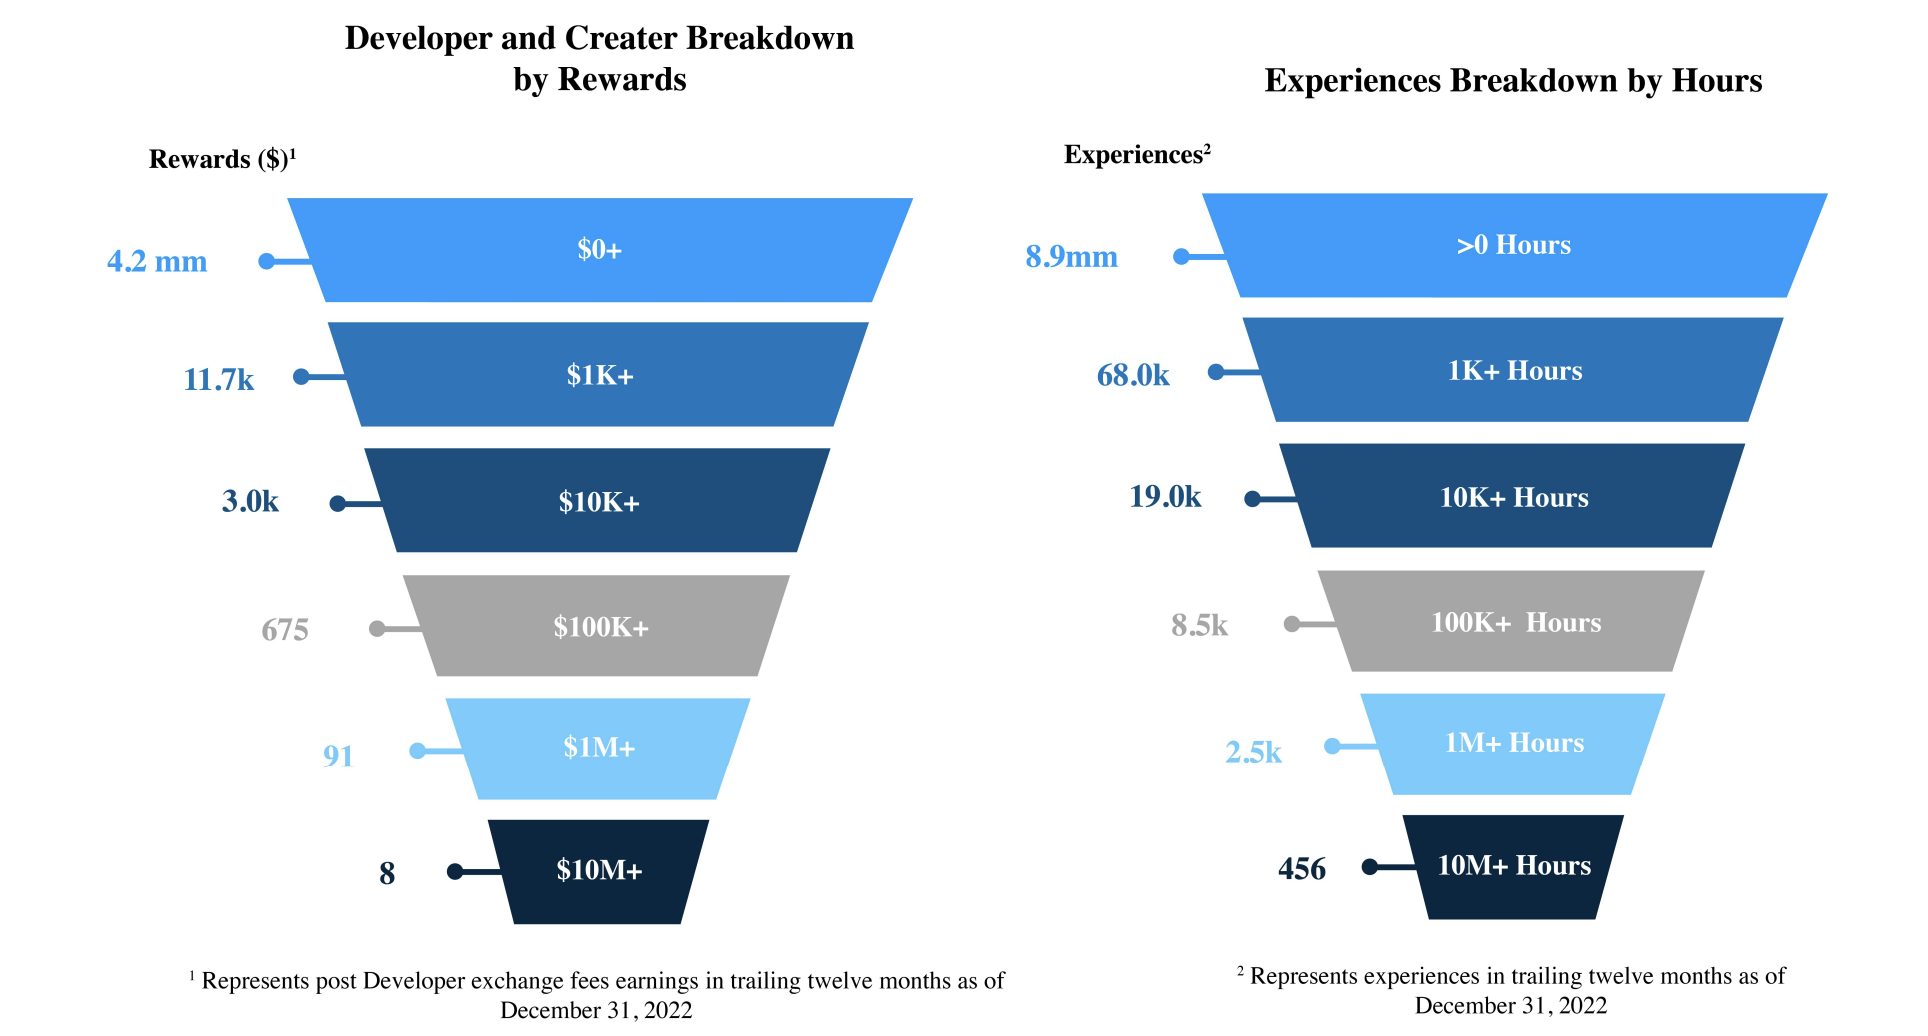
\includegraphics[width=.85\textwidth]{creators-numbers.png}}
  \caption{\anon{Creators numbers in 2022}}
  \label{fig:creators}

\end{figure}

\begin{quote}\em
  
Semantic subtyping
interprets types as sets of values, and subtyping as set
inclusion~\cite{GF05:GentleIntroduction}. This is aligned with the
\emph{minimize false positives} goal of \anon{Luau non-strict mode}, since
semantic subtyping only reports a failure of subtyping when there is a
value which inhabits the candidate subtype, but not the candidate
supertype.
For example, the program:
\begin{verbatim}
  local x : CFrame
    = CFrame.new()
  local y : Vector3 | CFrame
    = (math.random() < 0.5 ? CFrame.new() : Vector3.new())
  local z : Vector3 | CFrame
    = x * y
\end{verbatim}
cannot produce a run-time error, since multiplication of \verb|CFrame|s is overloaded:
\begin{verbatim}
  ((CFrame, CFrame) -> CFrame) & ((CFrame, Vector3) -> Vector3)
\end{verbatim}
In order to typecheck this program, we check that that type is a subtype of:
\begin{verbatim}
  (CFrame, Vector3 | CFrame) -> (Vector3 | CFrame)
\end{verbatim}
In the previous, syntax-driven, implementation of subtyping, this subtype check  would fail, resulting in a false positive.
We have now released an implementation of semantic subtyping, which does not suffer from this defect.
See our technical blog for more details~\anon{\cite{Jef22:SemanticSubtyping}}.

\end{quote}
%
In \anon{Luau}, we use a variant of semantic
subtyping~\cite{GF05:GentleIntroduction,FCB08:SemanticSubtyping,Ken21:DownDirty}. The
important properties of semantic subtyping are:
\begin{itemize}
\item there is a set $\Val$ of semantic values,
\item each type $T$ has a semantics $\sem{T} \subseteq \Val$,
\item $\UNKNOWN$ and $\NEVER$ types are interpreted as $\Val$ and $\emptyset$,
\item union and intersection types are interpreted as set union and intersection, and
\item subtyping $T <: U$ is interpreted as $\sem{T} \subseteq \sem{U}$.
\end{itemize}
The off-the-shelf presentation of semantic subtyping is \emph{set theoretic}~\cite[\S2.5]{GF05:GentleIntroduction}:
\[
  \sem{T_1} \subseteq \sem{T_2} \mbox{ if and only if }
  \mathcal{E}\sem{T_1} \subseteq \mathcal{E}\sem{T_2}
\]
where the most important case for $\mathcal{E}\sem{T}$ is function types:
\[
  \mathcal{E}\sem{S \fun T} = \mathcal{P}(\Val^2 \setminus (\sem{S} \times (\Val \setminus \sem{T})))
\]
The set theoretical requirement has some consequences:
  
\paragraph{All functions types $(\NEVER \fun T)$ are identified}

Consider
  \[\begin{array}{l}
    \mathcal{E}\sem{\NEVER \fun T_1} \\\quad
     = \mathcal{P}(\Val^2 \setminus (\sem{\NEVER} \times (\Val \setminus \sem{T_1}))) \\\quad
     = \mathcal{P}(\Val^2 \setminus (\emptyset \times (\Val \setminus \sem{T_1}))) \\\quad
     = \mathcal{P}(\Val^2) \\\quad
     = \mathcal{P}(\Val^2 \setminus (\emptyset \times (\Val \setminus \sem{T_2}))) \\\quad
     = \mathcal{P}(\Val^2 \setminus (\sem{\NEVER} \times (\Val \setminus \sem{T_2}))) \\\quad
     = \mathcal{E}\sem{\NEVER \fun T_2}
  \end{array}\]
  in particular, this means we cannot define a semantics-preserving function
  $\APPLY(T, U)$ such that:
  \[
    \APPLY(S \fun T, U) = T \mbox{ when } U <: S
  \]
  because there is a nasty case where $S$ is uninhabited. In this presentation,
  the $\APPLY$ function used in the rule for function application:
  \[
    \infer{
      D_1 : (\Gamma \vdash M : T) \\
      D_2 : (\Gamma \vdash N : U)
    }{
      \APP(D_1, D_2) : (\Gamma \vdash M(N) : \APPLY(T,U))
    }
  \]
  so we have to accept that in a set-theoretic model, the type rule for function
  application has corner cases for uninhabited types.

\paragraph{Union does not distributed through function types}
  
  Semantic subtyping gives a natural model of overloaded functions as intersections of arrows,
  for example the \anon{Roblox} API for matrices include an overloaded function
  which supports multiplication of both 2D (\verb|CFrame|) and 1D (\verb|Vector3|) matrices:
\begin{verbatim}
  CFrame.__mul : ((CFrame, CFrame) -> CFrame) & ((CFrame, Vector3) -> Vector3)
\end{verbatim}
  Overloaded functions are a key part of the \anon{Roblox} API, and we might expect that
  all function types can be presented as overloaded functions (that is intersections of arrows). We can do 
  that it we can distribute union through arrow:
  \[
    \sem{(S_1 \fun T_1) \cup (S_2 \fun T_2)}
    =
    \sem{(S_1 \cap S_2) \fun (T_1 \cup T_2)}
  \]
  For example:
  \[
    \sem{(\NUMBER? \fun \NUMBER) \cup (\STRING? \fun \STRING)}
    =
    \sem{\NIL \fun (\NUMBER \cup \STRING)}
  \]
  Unfortunately, set-theoretic models do not allow union to distributed through intersection,
  for example:
  \[\begin{array}{rcl}
    \{ (\texttt{1}, \NIL), (\texttt{"hi"}, \NIL) \} & \in & \mathcal{E}\sem{\NIL \fun (\NUMBER \cup \STRING)} \\
    \{ (\texttt{1}, \NIL), (\texttt{"hi"}, \NIL) \} & \not\in & \mathcal{E}\sem{\NUMBER? \fun \NUMBER} \\
    \{ (\texttt{1}, \NIL), (\texttt{"hi"}, \NIL) \} & \not\in & \mathcal{E}\sem{\STRING? \fun \STRING}
  \end{array}\]
  This is why type normalization for function types in set-theoretic models
  uses a conjunctive normal form of unions of intersections of functions e.g.~\cite[\S4.1.2]{Ken21:DownDirty}.

\paragraph{Set-theoretic mode support negatived types}
  
In addition, \anon{Luau} does not support negation of all types, but
only negation of \emph{test types}~\cite{CLNL22:OnTypeCases}, which
simplifies the model, by not requiring arbitrary type negation.  In
particular, since the model does not support negation of function
types, the normal form for function types is just overload functions,
not combinations of positive and negative function types.

\paragraph{Conclusions of this paper}

In summary there is a trade-off in semantic subtyping:
\begin{itemize}
  
\item \emph{set-theoretic} models, which are closer to the set-theoretic model
  of functions, and

\item \emph{pragmatic} models, which drop the set-theoretic requirement, and in return
  a)~do not have corner cases on the type of function application when the argument has uninhabited type, and
  b)~have overloaded functions (that is intersections of arrows) as the normal for function types.
  
\end{itemize}
\anon{Luau} chooses to adopt a pragmatic semantic subtyping model.

This paper shows how core \anon{Luau} pragmatic model is defined,
and how it formally (in Agda) proves pragmatic models.
There is the in the the full \anon{Luau} which is much bigger than the formally core language.

\section{Formal Treatment of Core \anon{Luau}}

This is a formal of a small core language. It has scalar types
($\NIL$, $\NUMBER$, $\BOOLEAN$ and $\STRING$), union and intersection types
(for example the optional $T?$ is a common shorthand $T \cup \NIL$),
and single-arity functions (like $\NUMBER? \fun \NUMBER$).
In this section why the core language can be formally, and in particularly
type normalization proved a algorithm for checking subtyping.

\subsection{Semantic Values for Core \anon{Luau}}

\begin{figure}
  
\[\begin{array}{rcl}
  v & ::= & s \mid (a \mapsto r) \\
  a & ::= & () \mid (v) \\
  r & ::= & \DIVERGE \mid \CHECK \mid (v) 
\end{array}\]
\caption{Semantic values}
\label{fig:semval}

\end{figure}

In this presentation, we present the minimal core of \anon{Luau},
which supports scalars and functions. This presentation ignores
tables, mutable features, and object objects.
We will ignore the details of scalar types,
and assume that there are scalar types, ranged over by $s$,
such as $\NIL$, $\BOOLEAN$, $\NUMBER$ and $\STRING$.

The types we are considering are:
\[
S, T ::= s \mid \UNKNOWN \mid \NEVER \mid S \fun T \mid S \cap T \mid S \cup T
\]
which are:
\begin{itemize}

\item the \emph{scalar types} $s$
  
\item the \emph{top type} $\UNKNOWN$,

\item the \emph{bottom type} $\NEVER$,

\item a \emph{function} type $S \fun T$,

\item an \emph{intersection} type $S \cap T$, and

\item a \emph{union} type $S \cup T$.

\end{itemize}
To give a semantic subtyping, we first declare the domain $\mathcal{D}$
of \emph{semantic values}, given by the grammar $v$ of Figure~\ref{fig:semval}.
Semantic values are:
\begin{itemize}
  
\item \emph{scalar values} $s$, and

\item \emph{function values} $a \mapsto r$,
  modeling a function that can can map an argument $a$ to
  a result $r$.

\end{itemize}
For example:
\begin{itemize}
  
\item $\TRUE$ and $\FALSE$ are values in $\BOOLEAN$,
\item $\TRUE$ and $\FALSE$ and $\NIL$ are values in the optional type $\BOOLEAN \cup \NIL$,
  and 
\item $(\TRUE) \mapsto (\FALSE)$ is a value in the function type $\BOOLEAN \fun \BOOLEAN$.

\end{itemize}
Scalar and error-suppressing values are relatively straightforward, but
functions are trickier. The case where a type-correct argument is
supplied and a type-correct result is returned is clean, for example:
\[
  ((\TRUE) \mapsto (\FALSE)) \in \sem{\BOOLEAN \fun \BOOLEAN}
\]
But there is also the case where a type-incorrect argument is
supplied, in which case there is no guarantee what is returned, for example:
\[
  ((5) \mapsto (37)) \in \sem{\BOOLEAN \fun \BOOLEAN}
\]
The type-correctness guarantee for results applies when a type-correct argument is provided:
\[
  ((\TRUE) \mapsto (37)) \not\in \sem{\BOOLEAN \fun \BOOLEAN}
\]
Those examples consider cases where one value is supplied as an argument,
and one is returned, but \anon{Luau} allows other cases.
\anon{Luau}, as is common in most functional languages, allows functions to diverge
(modeled in this semantics as $a \mapsto \DIVERGE$).,
for example:
\[
  ((\TRUE) \mapsto \DIVERGE) \in \sem{\BOOLEAN \fun \BOOLEAN}
\]
and:
\[
  ((5) \mapsto \DIVERGE) \in \sem{\BOOLEAN \fun \BOOLEAN}
\]
\anon{Luau} allows functions to check arguments,
(modeled in this semantics as $a \mapsto \CHECK$ when a checked fails),
for example:
\[
  ((5) \mapsto \CHECK) \in \sem{\BOOLEAN \fun \BOOLEAN}
\]
but:
\[
  ((\TRUE) \mapsto \CHECK) \not\in \sem{\BOOLEAN \fun \BOOLEAN}
\]
\anon{Luau} allows functions to be called without any arguments
(modeled in this semantics as $() \mapsto r$)
for example:
\[
  (() \mapsto (\FALSE)) \in \sem{\BOOLEAN \fun \BOOLEAN}
\]
and:
\[
  (() \mapsto \DIVERGE) \in \sem{\BOOLEAN \fun \BOOLEAN}
\]
and:
\[
  (() \mapsto \CHECK) \in \sem{\BOOLEAN \fun \BOOLEAN}
\]
The restriction on zero-argument function calls is that they are allowed to return
a $\CHECK$ (since they have been passed the wrong number of arguments)
but they are not just allowed to return arbitrary nonsense:
\[
  (() \mapsto (5)) \not\in \sem{\BOOLEAN \fun \BOOLEAN}
\]
At this point we have introduced the semantic values used by the \anon{Luau} type
system, and can turn the semantics of types, from which semantic subtyping follows.

\subsection{Semantics of Core \anon{Luau} Types}

\begin{figure}
  
\[\begin{array}{rcl}
  \sem{s} & = & \{ s \} \\
  \sem{\UNKNOWN} & = & \mathcal{D} \\
  \sem{\NEVER} & = & \emptyset \\
  \sem{S \fun T} & = & \{ a \mapsto (w) \mid w \in \sem{T} \} \cup {} \\
                    && \{ (v) \mapsto r \mid v \in \nsem{S} \} \cup {} \\
                    && \{ a \mapsto \DIVERGE \} \cup {} \\
                    && \{ () \mapsto \CHECK \} \\
  \sem{S \cap T} & = & \sem{S} \cap \sem{T} \\
  \sem{S \cup T} & = & \sem{S} \cup \sem{T} \\[\bigskipamount]
\end{array}\]
\caption{Semantics of types as sets of values}
\label{fig:typsem}

\end{figure}

The semantics of \anon{Luau} types are given in Fig~\ref{fig:typsem}.
This semantics is presented mechanically in Agda in~\anon{\cite{BJ23:agda-typeck}},
and we will give the most important results here.

For example, two of the important rules are for functions, in the case where
functions are called with argument values, and return result values.
The rules are:

\begin{itemize}
\item
  \textbf{Type-incorrect argument:}
  if $v \not\in \sem{S}$
  then $((v) \mapsto r) \in \sem{S \fun T}$
\item
  \textbf{Type-correct result:}
  if $w \in \sem{T}$
  then $(a \mapsto (w)) \in \sem{S \fun T}$
\end{itemize}
This is the same as the semantics of Coppo types~\cite{???}
as used in the fully abstract semantics of Lazy Lambda Calculus~\cite{???}
using Domain Theory In Logical Form~\cite{???}.
\[
  ((v) \mapsto (w)) \in \sem{S \fun T} \mbox{ if and only if }
  (v \in \sem{S}) \Rightarrow (w \in \sem{T})
\]
In order to give a constructive presentation of the semantics,
rather than usual negative presentation of $v \not\in \sem{S}$,
we give a positive presentation $v \in \nsem{S}$, as given in
Fig~\ref{fig:typnsem}.

\begin{figure}

\[\begin{array}{rcl}
  \nsem{s} & = & \{ t \mid s \neq t \} \\
  \nsem{\UNKNOWN} & = & \emptyset \\
  \nsem{\NEVER} & = & \mathcal{D} \\
  \nsem{S \fun T} & = & \{ s \} \cup {} \\
              && \{ () \mapsto (w) \mid w \in \nsem{T} \} \cup {} \\
              && \{ (v) \mapsto (w) \mid v \in \sem{T} \mid w \in \nsem{T} \} \cup {} \\
              && \{ (v) \mapsto \CHECK \mid v \in \sem{T} \} \\
  \nsem{S \cap T} & = & \nsem{S} \cup \nsem{T} \\
  \nsem{S \cup T} & = & \nsem{S} \cap \nsem{T}
\end{array}\]
\caption{Complemented semantics of types as sets of values}
\label{fig:typnsem}.

\end{figure}

It is routine to check that $\nsem{S \cap T}$ is a constructive
presentation of $\mathcal{D} \setminus \sem{S \cap T}$.

\begin{lemma}
  \label{lem:language-comp}
  $(v \in \nsem{T})$ if and only if $(v \not\in \sem{T})$.
\end{lemma}
\begin{proof}
  An proof by injunction on $T$ showings that $\sem{T}$ is the
  negative of $\nsem{T}$.
\end{proof}
Moreover there is a decision procedure for $v \in \sem{T}$ or $v \in \nsem{T}$.

\begin{lemma}
  \label{lem:language-dec}
  $(v \in \sem{T}) \lor (v \in \nsem{T})$.
\end{lemma}
\begin{proof}
  An proof by injunction on $T$, that for any $v$, either $v\in\sem{T}$ or $v\in\nsem{T}$.
\end{proof}

\subsection{Properties of Semantic Subtyping}

From the semantics of types as sets of semantic values,
semantic subtyping $S <: T$ is a proof than if $v \in \sem{S}$, then
$v \in \sem{T}$. Constructively this a dependent function:
\[
  (S <: T) \mbox{ if and only if } \forall v \st (v \in \sem{S}) \fun (v \in \sem{T})
\]
for example $\NUMBER <: \NUMBER?$ since:
\[
  \forall v \st (v \in \sem{\NUMBER}) \fun (v \in \sem{\NUMBER?})
\]
Subtyping can be viewed as a dependent function from $\nsem{T}$ to $\nsem{S}$

\begin{lemma}
  \label{lem:nsubtyp}
  $(S <: T)$ if and only if $\forall v \st (v \in \nsem{T}) \fun (v \in \nsem{S})$
\end{lemma}
\begin{proof}
  For ``if'', for any $v$, if $v \in \sem{S}$, then by Lemma~\ref{lem:language-dec}
  either $v \in \sem{T}$ or $v \in \nsem{T}$. In the first case, $v \in \sem{T}$ as needed.
  In the second case $v \in \nsem{T}$ and so by ``if'' hypothesis $v \in \nsem{S}$,
  but by Lemma~\ref{lem:language-comp} we have a contradiction from $v \in \sem{S}$ and $v \in \nsem{S}$.
  So we have established that $S <: T$.

  For ``only if'', for any $v$, if $v \in \nsem{T}$, then by Lemma~\ref{lem:language-dec}
  either $v \in \sem{S}$ or $v \in \nsem{S}$. 
  In the first case $v \in \sem{S}$ and so by ``only if'' hypothesis, $v \in \sem{T}$,
  but by Lemma~\ref{lem:language-comp} we have a contradiction from $v \in \sem{T}$ and $v \in \nsem{T}$.
  In the second case, $v \in \nsem{s}$ as needed.
  So we have established that $\forall v \st (v \in \nsem{T}) \fun (v \in \nsem{S})$.
\end{proof}
  
More interestingly is the constructive presentation of \emph{anti-subtyping} $S \not<: T$. Normally this is
presented negatively, but it can be read constructively since $S \not<: T$ is witnessed by
a value $v$ where $v \in \sem{S}$ but $v \in \nsem{T}$.
\[
  (S \not<: T) \mbox{ if and only if } \exists v \st (v \in \sem{S}) \land (v \in \nsem{T})
\]
for example $\NUMBER? \not<: \NUMBER$ since we can pick our witness $v$ to be $\NIL$:
\[
  \NIL \in \sem{\NUMBER?}
  \quad
  \NIL \in \nsem{\NUMBER}
\]
Now, by Lemma~\ref{lem:language-comp}, it is direct that $S \not<: T$ is a contradiction of $S <: T$:

\begin{lemma}
  $(S \not<: T) \fun \neg(S <: T)$
\end{lemma}
\begin{proof}
  The is a witness for $S \not<: T$, $v\in\sem{S}$ and $v\in\nsem{T}$,
  and so $S <: T$ and $v\in\sem{S}$ gives $v\in\sem{T}$.
  So Lemma~\ref{lem:language-comp} gives $v\in\nsem{T}$ and $v\in\sem{T}$
  are a contradiction is required.
\end{proof}
  
Unfortunately, this does not give a decision procedure for
subtyping, for the usual reason that it tricky to build an algorithm for
checking semantic subtyping, which requires type normalization~\cite{???}.
We will return to this in \S\ref{subsec:typnorm}.

It is direct to show that $<:$ is transitive.

\begin{lemma}
  $(S <: T) \land (T <: U) \fun (S <: U)$
\end{lemma}
\begin{proof}
  The there must be $f$ maps an argument with type $v \in\sem {S}$ to a result with type $v \in\sem {T}$,
  and there must be $g$ maps an argument with type $v \in\sem {T}$ to a result with type $v \in\sem {U}$.
  So $f;g$ maps an argument with type $v \in\sem {S}$ to a result with type $v \in\sem {U}$.
\end{proof}
More interestingly there is a dual property for $\not<:$.
Classically this is the same as transitivity, just stated in terms of $\not<:$ 
rather than $<:$. But constructively this is a choice function, that states that if
$S \not<: U$ then for any $T$ we have a witness for either $S \not<: T$ or $T \not<: U$.
For example $\NUMBER? \not<: \NUMBER$ (witnessed by $\NIL$), so for a mid-point $\STRING$
we have $\NIL\in\nsem{\STRING}$ which means we chose the constructive anti-subtype
$\NUMBER? \not<: \STRING$ witnessed by $\NIL\in\sem{\NUMBER?}$ and $\NIL\in\nsem{\STRING}$.

\begin{lemma}
  $(S \not<: U) \fun (S \not<: T) \lor (T \not<: U)$
\end{lemma}
\begin{proof}
  $(S \not<: U)$ must have a witness $v$ where
  $v \in \sem{S}$ and $v \in \nsem{U}$.
  Now by Lemma~\ref{lem:language-dec} (the decision procedure for type semantics)
  we either have $v \in \sem{T}$ or $v \in \nsem{T}$. In the first case,
  $v \in \sem{T}$ and $v \in \nsem{U}$, which witnesses $T \not<: U$.
  In the second case,
  $v \in \sem{S}$ and $v \in \nsem{T}$, which witnesses $S \not<: T$.
  In either case, we have a decision procedure for
  $(S \not<: T) \lor (T \not<: U)$.
\end{proof}

\subsection{Co- and Contra-variance of Subtyping for Functions}

We now turn to co- and contra-variant subtyping of functions.
These come in two flavors: when function types are introduced,
and when function types are eliminated.
When a function type is introduced, we
we check that the arguments respect contravariant subtyping,
and that the results respect covariant subtyping.

\begin{lemma}
  \label{lemma:intro-fun-variant}
  If $S' <: S$ and $T <: T'$
  then $(S \fun T) <: (S' \fun T')$
\end{lemma}
\begin{proof}
  If $u \in \sem{S \fun T}$
  then from Fig~\ref{fig:typsem}, either
  \begin{itemize}
  \item $u = (a \mapsto (w))$ and $w \in \sem{T}$, so $T <: T'$ implies
    $w \in \sem{T'}$, and so $(a \mapsto (w)) \in \sem{S' \fun T'}$,
  \item $u = ((v) \mapsto r)$ and $v \in \nsem{S}$, so $S' <: S$ and Lemma~\ref{lem:nsubtyp} implies
    $v \in \nsem{S'}$, and so $((v) \mapsto r) \in \sem{S' \fun T'}$,
  \item $u = (a \mapsto \DIVERGE)$, so $(a \mapsto \DIVERGE) \in \sem{S' \fun T'}$, or
  \item $u = () \mapsto \CHECK$, so $(() \mapsto \CHECK) \in \sem{S' \fun T'}$.
  \end{itemize}
  In any case, $u \in \sem{S' \fun T'}$.
\end{proof}
  
When a function type is eliminated, we
we check that the arguments reflect contravariant subtyping,
and that the results reflect covariant subtyping.

\begin{lemma}
  \label{lemma:elim-fun-variant}
  If $(S \fun T) <: (S' \fun T')$
  then $S' <: S$ and $T <: T'$
\end{lemma}
\begin{proof}
  If $v \in \nsem{S}$ then from Fig~\ref{fig:typsem}
  $((v) \mapsto \CHECK) \in \sem{S \fun T}$, so since 
  $(S \fun T) <: (S' \fun T')$, we have $((v) \mapsto \CHECK) \in \sem{S' \fun T'}$
  and so $v \in \nsem{S'}$. Thus, using Lemma~\ref{lem:nsubtyp},
  we have established $S' <: S$.

  If $w \in \sem{T}$ then from Fig~\ref{fig:typsem}
  $(() \mapsto (w)) \in \sem{S \fun T}$, so since 
  $(S \fun T) <: (S' \fun T')$, we have $(() \mapsto (w)) \in \sem{S' \fun T'}$
  and so $w \in \sem{T'}$. Thus we have established $T <: T'$.
\end{proof}

Note that these Lemmas rely on pragmatic semantic subtyping.
Lemma~\ref{lemma:intro-fun-variant} is true for set-theoretic
semantic subtyping, but Lemma~\ref{lemma:elim-fun-variant}
is only true for set-theoretic models when $S$ and $T$ are inhabited types.
In pragmatic semantic subtyping, we do not have special corner cases, in particular
Lemma~\ref{lemma:elim-fun-variant} is true for all types,
and does not require special cases about inhabitance.

\subsection{Distribution of Intersection and Union Over Functions}

Finally, we turn to cases where intersection and union distribute
through functions. Since \anon{Luau} uses intersections of functions as
types for overloaded functions, it is unsurprising that intersection does
not in general distribute through functions. For example:
\[
  (\BOOLEAN\fun\BOOLEAN) \cap (\NUMBER\fun\NUMBER)
\]
does not distribute to:
\[
  (\BOOLEAN\cup\NUMBER)\fun(\BOOLEAN\cap\NUMBER)
\]
For example:
\[\begin{array}{l}
  (\FALSE\mapsto\TRUE) \in \sem{(\BOOLEAN\fun\BOOLEAN) \cap (\NUMBER\fun\NUMBER)} \\
  (\FALSE\mapsto\TRUE) \in \nsem{(\BOOLEAN\cup\NUMBER)\fun(\BOOLEAN\cap\NUMBER)}
\end{array}\]
is a witness for:
\[\begin{array}{l}
  ((\BOOLEAN\fun\BOOLEAN) \cap (\NUMBER\fun\NUMBER)) \\\quad
  \not<:
  ((\BOOLEAN\cup\NUMBER)\fun(\BOOLEAN\cap\NUMBER))
\end{array}\]
Now in general we can not distribute intersection through functions,
on both the left and right, but we can distribute on just left, and just right.
This is similar to the situation with premonoids categories~\cite{??} which
are functorial on both sides, but are not binary functorials.

\begin{lemma} \mbox{}
  \begin{enumerate}
  \item $\sem{(S_1 \fun T) \cap (S_2 \fun T)} =
    \sem{(S_1 \cup S_2) \fun T}$
  \item $\sem{(S \fun T_1) \cap (S \fun T_2)} =
   \sem{S \fun (T_1 \cap T_2)}$
  \end{enumerate}
\end{lemma}
\begin{proof} \mbox{}
  \begin{enumerate}
    \item[(1$\Rightarrow$)]
  If $u \in \sem{S_1 \fun T} \cap \sem{S_2 \fun T}$,
  then from Fig~\ref{fig:typsem}, either
  \begin{itemize}
  \item $u = (a \mapsto (w))$ and $w \in \sem{T}$, 
    and so $(a \mapsto (w)) \in \sem{(S_1 \cup S_2) \fun T}$,
  \item $u = ((v) \mapsto r)$, $v \in \nsem{S_1}$
    and $v \in \nsem{S_2}$,
    so $v \in \nsem{S_1 \cup S_2}$,
    and so $((v) \mapsto r) \in \sem{(S_1 \cup S_2) \fun T}$,
  \item $u = (a \mapsto \DIVERGE)$, so $(a \mapsto \DIVERGE) \in \sem{(S_1 \cup S_2) \fun T}$, or
  \item $u = () \mapsto \CHECK$, so $(() \mapsto \CHECK) \in \sem{(S_1 \cup S_2) \fun T}$.
  \end{itemize}
  In any case, $u \in \sem{(S_1 \cup S_2) \fun T}$.

    \item[(1$\Leftarrow$)]
  If $u \in \sem{(S_1 \cup S_2) \fun T}$,
  then from Fig~\ref{fig:typsem}, either
  \begin{itemize}
  \item $u = (a \mapsto (w))$ and $w \in \sem{T}$, 
    and so $(a \mapsto (w)) \in \sem{S_1 \fun T} \cap \sem{S_2 \fun T}$,
  \item $u = ((v) \mapsto r)$, $v \in \nsem{S_1} \cap \nsem{S_2}$
    and so $((v) \mapsto r) \in \sem{S_1 \fun T} \cap \sem{S_2 \fun T}$,,
  \item $u = (a \mapsto \DIVERGE)$, so $(a \mapsto \DIVERGE) \in \sem{S_1 \fun T} \cap \sem{S_2 \fun T}$, or
  \item $u = () \mapsto \CHECK$, so $(() \mapsto \CHECK) \in \sem{S_1 \fun T} \cap \sem{S_2 \fun T}$.
  \end{itemize}
  In any case, $u \in \sem{S_1 \fun T} \cap \sem{S_2 \fun T}$.

    \item[(2$\Rightarrow$)]
  If $u \in \sem{S \fun T_1} \cap \sem{S \fun T_2}$,
  then from Fig~\ref{fig:typsem}, either
  \begin{itemize}
  \item $u = (a \mapsto (w))$, $w \in \sem{T_1}$ and $w \in \sem{T_2}$, 
    and so $(a \mapsto (w)) \in \sem{S \fun (T_1 \cap T_2)}$,
  \item $u = ((v) \mapsto r)$ and $v \in \nsem{S}$
    so $v \in \nsem{S}$,
    and so $((v) \mapsto r) \in \sem{S \fun (T_1 \cap T_2)}$,
  \item $u = (a \mapsto \DIVERGE)$, so $(a \mapsto \DIVERGE) \in \sem{S \fun (T_1 \cap T_2)}$, or
  \item $u = () \mapsto \CHECK$, so $(() \mapsto \CHECK) \in \sem{S \fun (T_1 \cap T_2)}$.
  \end{itemize}
  In any case, $u \in \sem{(S_1 \cup S_2) \fun T}$.

    \item[(2$\Rightarrow$)]
  If $u \in \sem{(S_1 \cup S_2) \fun T}$,
  then from Fig~\ref{fig:typsem}, either
  \begin{itemize}
  \item $u = (a \mapsto (w))$, $w \in \sem{T_1}$ and $w \in \sem{T_2}$, 
    and so $(a \mapsto (w)) \in \sem{S \fun T_1} \cap \sem{S \fun T_2}$,
  \item $u = ((v) \mapsto r)$ and $v \in \nsem{S}$
    so $v \in \nsem{S}$,
    and so $((v) \mapsto r) \in \sem{S \fun T_1} \cap \sem{S \fun T_2}$,
  \item $u = (a \mapsto \DIVERGE)$, so $(a \mapsto \DIVERGE) \in \sem{S \fun T_1} \cap \sem{S \fun T_2}$, or
  \item $u = () \mapsto \CHECK$, so $(() \mapsto \CHECK) \in \sem{S \fun T_1} \cap \sem{S \fun T_2}$.
  \end{itemize}
  In any case, $u \in \sem{S \fun T_1} \cap \sem{S \fun T_2}$.
  
  \end{enumerate}
  This provides cases.
\end{proof}

In contract, union does distribute over functions.

\begin{lemma}
  $\sem{(S_1 \fun T_1) \cup (S_2 \fun T_2)} =
   \sem{(S_1 \cap S_2) \fun (T_1 \cup T_2)}$
\end{lemma}
\begin{proof} \mbox{}
  \begin{enumerate}
    
  \item[($\Rightarrow$)]
  If $u \in \sem{S_1 \fun T_1} \cup \sem{S_2 \fun T_2}$,
  then from Fig~\ref{fig:typsem}, either
  \begin{itemize}
    
  \item $u = (a \mapsto (w))$, $w \in \sem{T_1}$, 
    and so $(a \mapsto (w)) \in \sem{(S_1 \cap S_2) \fun (T_1 \cup T_2)}$,

  \item $u = (a \mapsto (w))$, $w \in \sem{T_2}$, 
    and so $(a \mapsto (w)) \in \sem{(S_1 \cap S_2) \fun (T_1 \cup T_2)}$,

  \item $u = ((v) \mapsto r)$, $v \in \nsem{S_1}$
    and so $((v) \mapsto r) \in \sem{(S_1 \cap S_2) \fun (T_1 \cup T_2)}$,

  \item $u = ((v) \mapsto r)$, $v \in \nsem{S_2}$
    and so $((v) \mapsto r) \in \sem{(S_1 \cap S_2) \fun (T_1 \cup T_2)}$,

  \item $u = (a \mapsto \DIVERGE)$, so $(a \mapsto \DIVERGE) \in \sem{(S_1 \cap S_2) \fun (T_1 \cup T_2)}$, or
    
  \item $u = () \mapsto \CHECK$, so $(() \mapsto \CHECK) \in \sem{(S_1 \cap S_2) \fun (T_1 \cup T_2)}$.

  \end{itemize}
  In any case, $u \in \sem{(S_1 \cap S_2) \fun (T_1 \cup T_2)}$.

  \item[($\Leftarrow$)]
  If $u \in \sem{(S_1 \cap S_2) \fun (T_1 \cup T_2)}$,
  then from Fig~\ref{fig:typsem}, either
  \begin{itemize}
    
  \item $u = (a \mapsto (w))$, $w \in \sem{T_1}$, 
    and so $(a \mapsto (w)) \in \sem{S_1 \fun T_1} \cup \sem{S_2 \fun T_2}$,

  \item $u = (a \mapsto (w))$, $w \in \sem{T_2}$, 
    and so $(a \mapsto (w)) \in \sem{S_1 \fun T_1} \cup \sem{S_2 \fun T_2}$,

  \item $u = ((v) \mapsto r)$, $v \in \nsem{S_1}$
    and so $((v) \mapsto r) \in  \sem{S_1 \fun T_1} \cup \sem{S_2 \fun T_2}$,

  \item $u = ((v) \mapsto r)$, $v \in \nsem{S_2}$
    and so $((v) \mapsto r) \in \sem{S_1 \fun T_1} \cup \sem{S_2 \fun T_2}$,
    
  \item $u = (a \mapsto \DIVERGE)$, so $(a \mapsto \DIVERGE) \in \sem{S_1 \fun T_1} \cup \sem{S_2 \fun T_2}$, or
    
  \item $u = () \mapsto \CHECK$, so $(() \mapsto \CHECK) \in \sem{S_1 \fun T_1} \cup \sem{S_2 \fun T_2}$.

  \end{itemize}
  In any case, $u \in \sem{S_1 \fun T_1} \cup \sem{S_2 \fun T_2}$.

  \end{enumerate}
  This provides cases.
\end{proof}

Now, we have that the \anon{Luau} pragmatic semantic subtyping unions distinction,
the type normal for functions is:
\[
  (S_1 \fun T_1) \cap \cdots \cap (S_N \fun T_N)  
\] 
This the most important feature of type normalization.

\subsection{Type Normalization}
\label{subsec:typnorm}

\begin{figure}
  
\[\begin{array}{rcl}
  F & ::= & (S_1 \fun T_1) \cap \cdots \cap (S_m \fun T_m) \\
  N & ::= & F \cup s_1 \cup \cdots \cup s_n
\end{array}\]
\caption{Normalized types (when $m=0$ we consider $F$ to be $\NEVER$)}
\label{fig:ntypes}

\end{figure}

For Core \anon{Luau}, type nomalization is simplifier compared than sub-theoretic semantic subtyping,
as shown in Fig~\ref{fig:ntypes}. A normalized function type is a overloaded function, for example:
\[
  (\STRING? \fun \NUMBER?) \cap (\NUMBER \fun \NUMBER)
\]
The difficult part of normalized types is function types, but we also consider normalized types with scalars
for example optional $\NUMBER$
\[
  \NUMBER \cup \NIL
\]
or a function type that may be a function type or a scalar type for example
the overloaded function or optional $\NUMBER$:
\[
  ((\STRING? \fun \NUMBER?) \cap (\NUMBER \fun \NUMBER)) \cup \NUMBER \cup \NIL
\]

\begin{lemma} \label{lem:funun}
  For any normalized function type $F_1$ and $F_2$,
  there is a normalized function type $F_0$,
  where $\sem{F_1} \cup \sem{F_2}$ is $\sem{F_0}$,
\end{lemma}

\begin{proof}
  xxx
\end{proof}

\begin{lemma}
  For any function type there is equivalent normalized function type.
\end{lemma}

\begin{proof}
  Cases:
  \begin{itemize}
  \item $\NEVER$: Is normalized function type when $m$ is zero.
  \item $S \fun T$: Is a normalized function type when $m$ is $1$ and $(S_1 \fun T_1)$ is $(S \fun T)$.
  \item $S \cap T$: By indiction we have normalized function types,
    and by definition normalized function types support intersection.
  \item $S \cup T$: By indiction we have normalized function types,
    and by Lemma~\ref{lem:funun} normalized function types support union.
  \end{itemize}
  This is an induction where the only tricky case is union, which is given by Lemma~\ref{lem:funun}.
\end{proof}

\begin{lemma}
  For any type there is equivalent normalized type.
\end{lemma}

\begin{proof}
   xxx
\end{proof}

\section{Implementation of Full \anon{Luau}}

Stuff features
\begin{itemize}
\item Functions with arity.
\item Functions with vararg.
\item Tables.
\item Tables with indexers.
\item Tables with tagged unions.
\item Singleton types.
\item Genetics.
\item FBI.
\end{itemize}
Stuff imp's
\begin{itemize}
\item How we implement type normalization.
\item Aim for type inference in 16ms.
\item Telemetry with very few \verb|CodeTooComplex|.
\item SAT solves.
\end{itemize}

\section{Further work}

\bibliographystyle{ACM-Reference-Format}
\bibliography{bibliography}

\end{document}
